\documentclass[11pt]{article}
\usepackage[a4paper,margin=27mm,headheight=15pt]{geometry}
\usepackage[T1]{fontenc}
\usepackage[utf8]{inputenc}
\IfFileExists{libertinus.sty}{\usepackage{libertinus}}{\usepackage{lmodern}}
\usepackage{microtype}
\usepackage{amsmath,amssymb,amsthm,mathtools,bm}
\usepackage{booktabs,longtable,tabularx,array}
\usepackage{graphicx}
\usepackage{enumitem}
\usepackage{xcolor}
\usepackage{fancyhdr}
\usepackage{hyperref}
\usepackage[nameinlink,capitalise,noabbrev]{cleveref}
\usepackage{xurl}
\allowdisplaybreaks

\definecolor{linkblue}{RGB}{32,72,116}
\definecolor{darkgreen}{RGB}{33,94,68}
\hypersetup{
 colorlinks=true,linkcolor=linkblue,citecolor=darkgreen,urlcolor=linkblue,
 pdftitle={Total Positivity and Cartwright Geometry in the Fabius--Rvachev Dyadic Sinc Product},
 pdfauthor={OpenAI},
 pdfsubject={New structural results for the Fabius function and Rvachev up function}
}
\pagestyle{fancy}
\fancyhf{}
\fancyhead[L]{\small Fabius--Rvachev total positivity and Cartwright geometry}
\fancyhead[R]{\small\thepage}
% Canonical project-wide mathematical notation.
% Canonical mathematical notation for active FabiusFunction LaTeX documents.
%
% This file is intentionally a plain TeX input rather than a LaTeX package.
% Every standalone document loads it by an explicit path relative to that
% document's directory; included fragments inherit the definitions from their
% root document.  Keep this file independent of document layout and metadata.
%
% Contract:
%   * one command has one mathematical meaning throughout the active corpus;
%   * names encode semantic roles rather than a document-local choice of letter;
%   * visually similar but differently normalized objects have different print;
%   * every command below is defined normatively in the notation catalogue.
%
% The active corpus excludes docs/archive/.  Historical sources may retain
% their original notation only inside an explicitly labelled quotation.

\makeatletter
\@ifundefined{mathbb}{%
  \PackageError{fabius-notation}{The amssymb package must be loaded first}%
    {Load amsmath and amssymb before inputting fabius-notation.tex.}%
}{}
\@ifundefined{operatorname}{%
  \PackageError{fabius-notation}{The amsmath package must be loaded first}%
    {Load amsmath before inputting fabius-notation.tex.}%
}{}
\makeatother

% Version stamp used by the catalogue and by static audits.
\newcommand{\FabiusNotationVersion}{2026-08-31}

% Number systems.  NaturalNumbers is explicitly the nonnegative convention.
\newcommand{\NaturalNumbers}{\mathbb{N}_{0}}
\newcommand{\PositiveIntegers}{\mathbb{N}_{>0}}
\newcommand{\IntegerNumbers}{\mathbb{Z}}
\newcommand{\RationalNumbers}{\mathbb{Q}}
\newcommand{\RealNumbers}{\mathbb{R}}
\newcommand{\ComplexNumbers}{\mathbb{C}}
\newcommand{\ExtendedRealNumbers}{\overline{\mathbb{R}}}

% The three principal Fabius--Rvachev functions.  Subscripts are deliberate:
% a bare F and a calligraphic F have several unrelated uses in the corpus.
\newcommand{\FabiusBounded}{F_{\mathrm{bd}}}
\newcommand{\FabiusGlobal}{F_{\mathrm{gl}}}
\newcommand{\FabiusQuantile}{Q_{F}}
\newcommand{\FabiusClampedQuantile}{Q_{F,\mathrm{cl}}}
\newcommand{\RvachevUp}{\operatorname{up}}

% Constants, elementary operators, and delimiters.
\newcommand{\EulerE}{\mathrm{e}}
\newcommand{\ImaginaryUnit}{\mathrm{i}}
\newcommand{\Differential}{\mathop{}\!\mathrm{d}}
\newcommand{\AbsoluteValue}[1]{\left\lvert #1\right\rvert}
\newcommand{\Norm}[1]{\left\lVert #1\right\rVert}
\newcommand{\Floor}[1]{\left\lfloor #1\right\rfloor}
\newcommand{\Ceiling}[1]{\left\lceil #1\right\rceil}
\newcommand{\FractionalPart}[1]{\left\{#1\right\}}
\newcommand{\PositivePart}[1]{\left(#1\right)_{+}}
\newcommand{\IndicatorOf}[1]{\mathbf{1}_{#1}}
\newcommand{\SetOf}[1]{\left\{#1\right\}}
\newcommand{\InnerProduct}[1]{\left\langle #1\right\rangle}
\newcommand{\CardinalityOf}[1]{\left\lvert #1\right\rvert}
\newcommand{\DefinitionEquals}{\mathrel{\coloneqq}}
\newcommand{\Sign}{\operatorname{sgn}}
\newcommand{\IdentityOperator}{\operatorname{id}}
\newcommand{\SpanOperator}{\operatorname{span}}
\newcommand{\TraceOperator}{\operatorname{tr}}
\newcommand{\RankOperator}{\operatorname{rank}}
\newcommand{\DiagonalOperator}{\operatorname{diag}}
\newcommand{\ResidueOperator}{\operatorname*{Res}}
\newcommand{\LeastCommonMultiple}{\operatorname{lcm}}
\newcommand{\OrderOperator}{\operatorname{ord}}
\newcommand{\PrincipalLogarithm}{\operatorname{Log}}
\newcommand{\FallingFactorial}[2]{\left(#1\right)^{\underline{#2}}}
\newcommand{\RisingFactorial}[2]{\left(#1\right)^{\overline{#2}}}

% Support, topology, convolution, and metric notation.
\newcommand{\SupportOperator}{\operatorname{supp}}
\newcommand{\SupportOf}[1]{\SupportOperator\!\left(#1\right)}
\newcommand{\TopologicalSupportOf}[1]{\operatorname{tsupp}\!\left(#1\right)}
\newcommand{\Convolution}{\mathbin{*}}
\newcommand{\MetricDistance}{\operatorname{dist}}
\newcommand{\TotalVariationDistance}{d_{\mathrm{TV}}}

% Probability.  Equality and convergence in law are not metric distance.
\newcommand{\Probability}{\mathbb{P}}
\newcommand{\Expectation}{\mathbb{E}}
\newcommand{\Variance}{\operatorname{Var}}
\newcommand{\Covariance}{\operatorname{Cov}}
\newcommand{\LawOperator}{\operatorname{Law}}
\newcommand{\LawOf}[1]{\LawOperator\!\left(#1\right)}
\newcommand{\EqualInLaw}{\mathrel{\overset{\mathrm{law}}{=}}}
\newcommand{\ConvergesInLaw}{\mathrel{\xrightarrow{\mathrm{law}}}}

% Fourier and integral transforms.  The printed labels expose normalization.
% FourierTwoPi uses exp(-2*pi*i*x*xi); FourierAngular uses exp(-i*x*omega).
\newcommand{\FourierTwoPi}[1]{\widehat{#1}_{\,2\pi}}
\newcommand{\FourierAngular}[1]{\widehat{#1}_{\,\mathrm{ang}}}
\newcommand{\LaplaceTransformSymbol}{\mathcal{L}}
\newcommand{\MellinTransformSymbol}{\mathcal{M}}
\newcommand{\LaplaceTransformOf}[1]{\LaplaceTransformSymbol\!\left[#1\right]}
\newcommand{\MellinTransformOf}[1]{\MellinTransformSymbol\!\left[#1\right]}
\newcommand{\MomentGeneratingFunction}[1]{M_{#1}}
\newcommand{\CharacteristicFunction}[1]{\varphi_{#1}}

% The two standard sinc functions must never share one symbol.
\newcommand{\SincRad}{\operatorname{sinc}_{\mathrm{rad}}}
\newcommand{\SincPi}{\operatorname{sinc}_{\pi}}

% Binary arithmetic and Thue--Morse notation.
\newcommand{\BinaryDigitSum}{\operatorname{wt}_{2}}
\newcommand{\ThueMorseSignSymbol}{\varepsilon}
\newcommand{\ThueMorseSign}[1]{\varepsilon_{#1}}
\newcommand{\PadicValuation}[1]{\nu_{#1}}
\newcommand{\TwoAdicValuation}{\nu_{2}}

% q-series notation.  Every base is an explicit argument.
\newcommand{\QPochhammer}[3]{\left(#1;#2\right)_{#3}}
\newcommand{\GaussianBinomial}[3]{%
  \genfrac{[}{]}{0pt}{}{#1}{#2}_{#3}%
}
\newcommand{\QInteger}[2]{\left[#1\right]_{#2}}

% Named special functions.
\newcommand{\Polylogarithm}{\operatorname{Li}}
\newcommand{\LambertW}{W}
\newcommand{\GammaFunction}{\Gamma}
\newcommand{\RiemannZeta}{\zeta}

% Asymptotics.  BigO and LittleO are operator tokens for existing formula
% grammar; prefer the At forms so that the limiting regime is printed.
\newcommand{\BigO}{\mathcal{O}}
\newcommand{\LittleO}{o}
\newcommand{\BigOAt}[2]{\mathcal{O}_{#2}\!\left(#1\right)}
\newcommand{\LittleOAt}[2]{o_{#2}\!\left(#1\right)}

\renewcommand{\headrulewidth}{0.35pt}
\setcounter{tocdepth}{2}
\setcounter{secnumdepth}{3}
\setlist{itemsep=2pt,topsep=5pt}
\numberwithin{equation}{section}

\newtheorem{theorem}{Theorem}[section]
\newtheorem{proposition}[theorem]{Proposition}
\newtheorem{lemma}[theorem]{Lemma}
\newtheorem{corollary}[theorem]{Corollary}
\newtheorem{conjecture}[theorem]{Conjecture}
\theoremstyle{definition}
\newtheorem{definition}[theorem]{Definition}
\newtheorem{example}[theorem]{Example}
\newtheorem{problem}[theorem]{Problem}
\theoremstyle{remark}
\newtheorem{remark}[theorem]{Remark}
\newtheorem{warning}[theorem]{Warning}


\title{\textbf{Total Positivity and Cartwright Geometry\\in the Fabius--Rvachev Dyadic Sinc Product}\\[0.55em]
\large Laguerre--Pólya structure, multiplier sequences, exact Thue--Morse sign interpolation, and a geometric-scale deformation}
\author{A frontier research report based on the \texttt{ProveIt} Fabius-function corpus}
\date{30 August 2026\\Repository snapshot \texttt{fc4b8868fcf57cc534d22f438d940ec65ebbe767}}

\begin{document}
\maketitle

\begin{abstract}
The Fourier transform of Rvachev's compactly supported up function is the dyadic sinc product
\[
 \widehat{\RvachevUp}(z)=\prod_{j=0}^{\infty}\SincRad\!\left(\frac{\pi z}{2^j}\right).
\]
The existing \texttt{ProveIt} corpus develops its probabilistic construction, exact dyadic arithmetic, $q$-binomial and Thue--Morse identities, moments, Legendre expansions, endpoint and inverse-function asymptotics, Lambert-$W$ inversion, and several spectral and Hankel directions.  This report takes a different route.  Under the imaginary square-root substitution
\[
 H(x):=\widehat{\RvachevUp}\!\left(\frac{\ImaginaryUnit\sqrt{x}}{\pi}\right)
      =\prod_{j=0}^{\infty}\frac{\sinh(2^{-j}\sqrt{x})}{2^{-j}\sqrt{x}},
\]
the oscillatory sinc product becomes a genus-zero entire function whose zeros are all negative.  Its Taylor coefficients are scaled even moments of $\RvachevUp$.  This observation places those moments in the Laguerre--Pólya, Pólya-frequency, multiplier-sequence, Jensen-polynomial, and Poisson-binomial theories simultaneously.

The main proved results are as follows.  The coefficient sequence of $H$ is PF$_\infty$; the factorially rescaled sequence is a classical multiplier sequence; every shifted Jensen polynomial is real-rooted with negative zeros; and the even moments satisfy a new two-sided adjacent-moment inequality.  The coefficients admit exact Bell-polynomial and Bernoulli recurrences driven by the Lambert factors $(1-4^{-m})^{-1}$.  More generally, a one-parameter family $H_q$ has the same structure for every $0<q<1$, with explicit power sums and coefficient asymptotics.  A Bernoulli-sum representation gives an implicit saddle formula and yields
\[
 n^2a_n(q)^{1/n}\longrightarrow \frac{\EulerE^2}{4(1-\sqrt q)^2},
 \qquad
 n^2\frac{a_{n+1}(q)}{a_n(q)}\longrightarrow \frac{1}{4(1-\sqrt q)^2}.
\]
For $q=1/4$ these limits are $\EulerE^2$ and $1$.

On the original Fourier side, the zero at the nonzero integer $N$ has multiplicity $\nu_2(N)+1$.  Consequently the multiplicity-weighted positive zero count is exactly $2N-s_2(N)$, and, more strikingly,
\[
 \Sign\widehat{\RvachevUp}(x)=\ThueMorseSign{\Floor{x}}
 \qquad(x>0,\ x\notin\IntegerNumbers).
\]
Thus the sinc product analytically interpolates the Thue--Morse word by its signs on consecutive unit intervals.  We also determine its Cartwright indicator and extend the zero-count/sign theorem to integer dilation bases.  The report closes with conjectural Hermite limits for Jensen polynomials, a log-periodic coefficient transseries expected to be dual to the known endpoint fluctuation, arithmetic questions for rational $q$, and concrete formalization targets.

All claims labeled theorem, proposition, lemma, or corollary are proved here.  Claims labeled conjecture or problem are deliberately unproved.  The arrival-time novelty screen was incomplete: the pinned corpus already contained overlapping Laguerre--P\'olya, PF$_\infty$, shifted-Jensen, zero-count, and sign material.  Accordingly, ``new'' below describes report-local deductions and packaging after the corrected crosswalk in \cref{sec:audit}; it is neither a claim of absence from the repository nor a claim of exhaustive priority over the literature.
\end{abstract}

\tableofcontents
\newpage

\section{Corpus audit, scope, and novelty controls}\label{sec:audit}

\subsection{Pinned recursive audit}

The repository was audited recursively at commit
\[
 \texttt{fc4b8868fcf57cc534d22f438d940ec65ebbe767}
\]
(the then-current head of \texttt{main}).  GitHub's code index returned 87 files with extension \texttt{.tex} below \texttt{Analysis/FabiusFunction/docs}.  The audit included nested source-paper transcriptions, primary expositions, archived variants, generated numerical fragments, and the large collection of semi-formalized frontier drafts.  Duplicated or near-duplicated archived versions were still checked for theorem-level differences; they were not counted as independent evidence of novelty.

The material falls into the following overlapping families.
\begin{longtable}{p{0.25\textwidth}p{0.68\textwidth}}
\toprule
Family & Material already present and therefore excluded as a principal novelty claim \\
\midrule
\endhead
Foundations & Definitions of the bounded and global Fabius functions, Rvachev's up function, convolution/random-series constructions, smoothness, support, partition of unity, Fourier inversion, and source papers by Arias de Reyna and others.\\
Dyadic arithmetic & Exact values at dyadic rationals, half moments, denominator and integrality results, executable recurrences, terminating Taylor formulae, and Lean formalization architecture.\\
$q$-calculus and Thue--Morse & Finite $q$-Pochhammer products, Gaussian binomial coefficients at base $1/2$, Thue--Morse cancellations, finite difference stencils, and exact global expansions.\\
Endpoint asymptotics & Small-argument Fabius asymptotics, all-orders corrections, periodic Gamma--zeta fluctuations, Lambert-$W$ inversion, and inverse-Fabius expansions.\\
Transforms and products & Infinite sinc products, Mellin/Fourier transforms, moment generating functions, integral transforms, and related Bernoulli/Bell machinery.\\
Approximation and sampling & Dyadic comb sums, Lagrange and Hermite interpolation, Runge phenomena, quadrature, antiderivatives, and fractional-calculus directions.\\
Orthogonal representations & Legendre expansions of $\RvachevUp$, finite synthesis of polynomials by shifted up functions, and Lagrange/Legendre closed-loop substitutions.\\
Recent frontier drafts & Spectral moments, valuation packages, Gamma and zeta modes, Stieltjes and Hankel structures, Padé questions, and several compiled frontier surveys.\\
\bottomrule
\end{longtable}

The arrival-time exact-phrase search missed existing repository overlap.  At
the pinned checkpoint, Part~V of \texttt{Frontier\_Compilations} already
contained the matching Laguerre--P\'olya/PF$_\infty$/shifted-Jensen layer,
with zero-count and sign material elsewhere in the same consolidated volume.
Those strands are inherited baseline here.  The targeted external search
still included the classical P\'olya--Schur paper, the
Aissen--Edrei--Schoenberg--Whitney characterization of totally positive
sequences, modern Jensen-polynomial work, Cartwright-class literature, and
the principal Fabius papers.  The present report remains useful as a unified
proof-oriented treatment, but its novelty claims must be read subject to this
corrected repository crosswalk.

\subsection{The linked layer developed here}

The report does not merely attach classical terminology to a known product.
Its linked deductions and useful joint packaging are the following.
\begin{enumerate}[leftmargin=2.2em]
\item The imaginary square-root transform identifies the scaled Rvachev moment sequence with the elementary symmetric functions of an explicit dyadic spectral alphabet.
\item This gives PF$_\infty$ Toeplitz total positivity and an exact multiplier sequence, hence hyperbolicity of every shifted Jensen polynomial.
\item Combining multiplier Turán inequalities with ordinary moment log-convexity gives a sharp asymptotic-width sandwich for three consecutive Rvachev moments.
\item The same alphabet gives a Poisson-binomial saddle model, from which coefficient root and ratio limits follow.
\item The dyadic zero divisor gives an exact sign interpolation of the Thue--Morse sequence on all nonintegral positive arguments.
\item A geometric $q$-deformation and an arbitrary-scale theorem reveal which parts are consequences of positivity and which parts are genuinely binary.
\end{enumerate}

\section{Normalization and the decisive transform}\label{sec:normalization}

We use
\[
 \SincRad z=\begin{cases}\sin z/z,&z\ne0,\\1,&z=0.\end{cases}
\]
The Fourier convention is the one used in the source corpus:
\[
 \widehat f(z)=\int_{\RealNumbers}f(t)\EulerE^{-2\pi\ImaginaryUnit zt}\,\Differential t.
\]
The normalized up function has integral one and Fourier transform
\begin{equation}\label{eq:up-product}
 \widehat{\RvachevUp}(z)=\prod_{j=0}^{\infty}\SincRad\!\left(\frac{\pi z}{2^j}\right).
\end{equation}
Let
\begin{equation}\label{eq:moments}
 c_n:=\int_{-1}^{1}t^{2n}\RvachevUp(t)\,\Differential t\qquad(n\ge0).
\end{equation}
Evenness gives the Maclaurin expansion
\begin{equation}\label{eq:fourier-moment-expansion}
 \widehat{\RvachevUp}(z)=\sum_{n=0}^{\infty}(-1)^n\frac{c_n}{(2n)!}(2\pi z)^{2n}.
\end{equation}

\begin{definition}[Imaginary square-root transform]\label{def:H}
Define the entire function
\begin{equation}\label{eq:H-def}
 H(x):=\widehat{\RvachevUp}\!\left(\frac{\ImaginaryUnit\sqrt{x}}{\pi}\right)
 =\prod_{j=0}^{\infty}\frac{\sinh(2^{-j}\sqrt{x})}{2^{-j}\sqrt{x}}
 =:\sum_{n=0}^{\infty}a_nx^n.
\end{equation}
Each factor is interpreted by its power series, so no choice of a square-root branch remains.
\end{definition}

Substitution in \eqref{eq:fourier-moment-expansion} immediately gives the first bridge.
\begin{proposition}[Moment coefficient identity]\label{prop:moment-coeff}
For every $n\ge0$,
\begin{equation}\label{eq:a-c}
 a_n=\frac{4^n c_n}{(2n)!}.
\end{equation}
In particular all $a_n$ are positive rational numbers.
\end{proposition}
\begin{proof}
At $z=\ImaginaryUnit\sqrt{x}/\pi$, the two signs $(-1)^n$ and $\ImaginaryUnit^{2n}=(-1)^n$ cancel, while $(2\pi z)^{2n}=(-4x)^n$.  Equation \eqref{eq:a-c} follows.  Positivity is also immediate from \eqref{eq:moments}; rationality is known from the moment recurrence, and will follow again from \cref{sec:bell}.
\end{proof}

The elementary Weierstrass product
\begin{equation}\label{eq:sinh-product}
 \frac{\sinh y}{y}=\prod_{k=1}^{\infty}\left(1+\frac{y^2}{\pi^2k^2}\right)
\end{equation}
turns \eqref{eq:H-def} into
\begin{equation}\label{eq:H-double-product}
 H(x)=\prod_{j=0}^{\infty}\prod_{k=1}^{\infty}
       \left(1+\frac{4^{-j}x}{\pi^2k^2}\right).
\end{equation}
The double product converges locally uniformly because
\[
 \sum_{j\ge0}\sum_{k\ge1}\frac{4^{-j}}{\pi^2k^2}
 =\frac1{6}\frac1{1-1/4}=\frac29.
\]
This positive genus-zero product is the structural pivot of the report.

\section{The dyadic zero divisor and exact Thue--Morse sign interpolation}\label{sec:zeros}

Let $\nu_2(N)$ be the exponent of $2$ in the prime factorization of the positive integer $N$, and let $s_2(N)$ be its binary digit sum.  Write
\[
 \ThueMorseSign{N}:=(-1)^{s_2(N)}
\]
for the $\{+1,-1\}$ form of the Thue--Morse sequence.

\begin{theorem}[Exact zero multiplicities]\label{thm:zero-multiplicity}
For every nonzero integer $N$,
\begin{equation}\label{eq:zero-order}
 \OrderOperator_{z=N}\widehat{\RvachevUp}(z)=\nu_2(\AbsoluteValue N)+1.
\end{equation}
Equivalently, $H$ has a zero at $-\pi^2N^2$ of multiplicity $\nu_2(N)+1$ and has no other zeros.
\end{theorem}
\begin{proof}
The $j$th factor of \eqref{eq:up-product} vanishes at $z=N$ precisely when $N/2^j$ is a nonzero integer, i.e. when $0\le j\le\nu_2(N)$.  Each such sine zero is simple, and all other factors are nonzero.  This proves \eqref{eq:zero-order}.  The statement for $H$ follows either by substitution or directly from \eqref{eq:H-double-product}.
\end{proof}

\begin{theorem}[Exact zero count and digit-sum discrepancy]\label{thm:zero-count}
Let $M=\Floor R$ for $R\ge0$, and count zeros with multiplicity.  The number of positive zeros of $\widehat{\RvachevUp}$ in $(0,R]$ is
\begin{equation}\label{eq:positive-zero-count}
 Z_+(R)=2M-s_2(M).
\end{equation}
The number of nonzero zeros in $[-R,R]$ is
\begin{equation}\label{eq:total-zero-count}
 Z(R)=4M-2s_2(M).
\end{equation}
\end{theorem}
\begin{proof}
By \cref{thm:zero-multiplicity},
\[
 Z_+(R)=\sum_{n=1}^{M}(\nu_2(n)+1)=M+\nu_2(M!).
\]
Legendre's identity $\nu_2(M!)=M-s_2(M)$ proves \eqref{eq:positive-zero-count}.  Evenness of the product gives \eqref{eq:total-zero-count}.
\end{proof}

The parity consequence is stronger than a counting curiosity.
\begin{theorem}[Thue--Morse sign interpolation]\label{thm:sign-interpolation}
For every $x>0$ that is not an integer,
\begin{equation}\label{eq:sign-interpolation}
 \Sign\widehat{\RvachevUp}(x)=\ThueMorseSign{\Floor{x}}=(-1)^{s_2(\Floor{x})}.
\end{equation}
Thus $\widehat{\RvachevUp}$ has constant sign on every open unit interval $(N,N+1)$, and those signs spell the Thue--Morse word exactly.
\end{theorem}
\begin{proof}
The product is positive on $(0,1)$.  Passing a real zero of multiplicity $m$ changes the sign exactly when $m$ is odd.  Hence the sign on $(N,N+1)$ equals
\[
 (-1)^{Z_+(N)}=(-1)^{2N-s_2(N)}=(-1)^{s_2(N)}.
\]
There are no other real zeros, so the sign is constant on the interval.
\end{proof}

\begin{remark}
This theorem realizes Thue--Morse without inserting its coefficients by hand: the word is the parity shadow of the collision multiplicities among the dyadic sine factors.  The usual product identity for Thue--Morse describes cancellation in a finite exponential sum; \cref{thm:sign-interpolation} instead describes the global sign geometry of an entire Fourier transform.
\end{remark}

\begin{figure}[htbp]
\centering
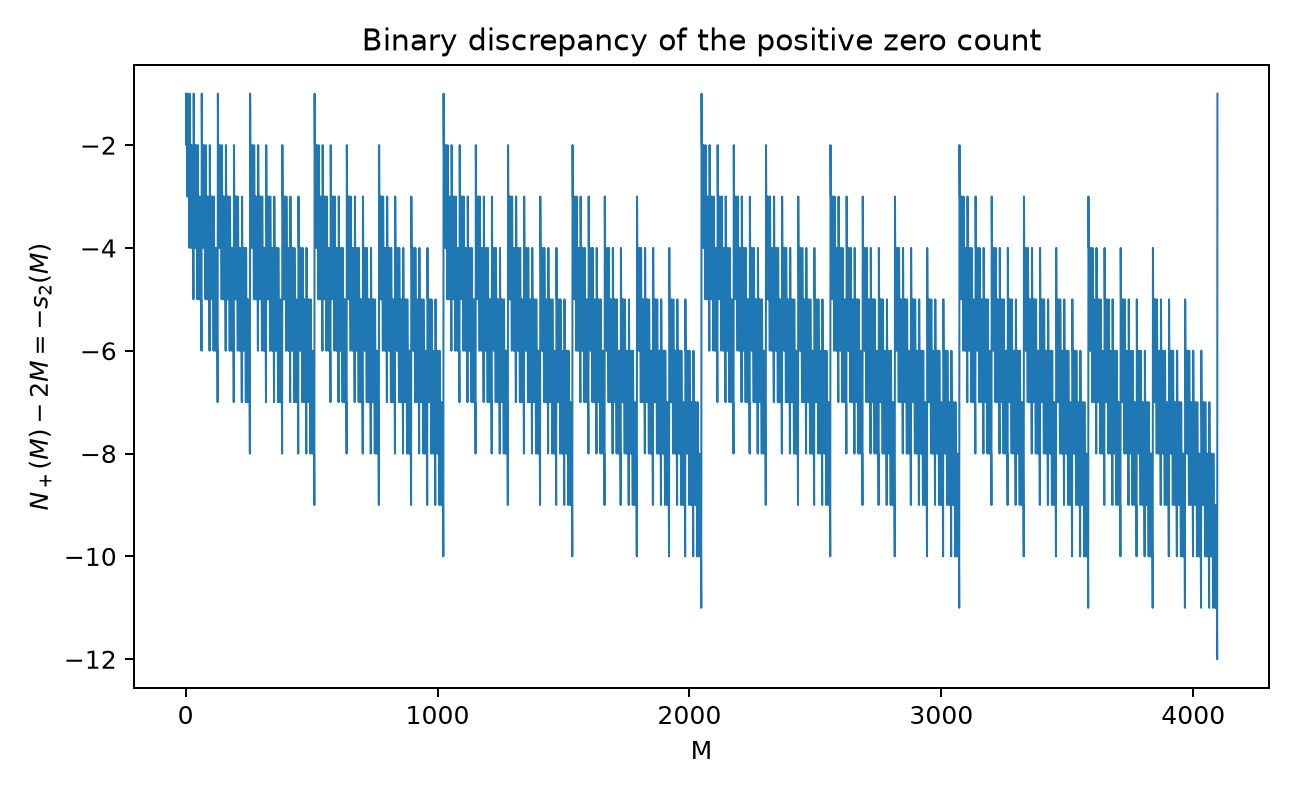
\includegraphics[width=0.88\textwidth]{figures/zero_count_binary_discrepancy.png}
\caption{The exact discrepancy $Z_+(M)-2M=-s_2(M)$.  The nested sawtooth pattern is not numerical noise: every plotted value is an integer identity.}
\label{fig:zero-discrepancy}
\end{figure}

\subsection{Integer-base generalization}

For an integer $b\ge2$, define
\begin{equation}\label{eq:base-b-product}
 \Phi_b(z):=\prod_{j=0}^{\infty}\SincRad\!\left(\frac{\pi z}{b^j}\right).
\end{equation}
Let $\nu_b(N)=\max\{j:b^j\mid N\}$ and let $s_b(N)$ be the sum of the base-$b$ digits of $N$.

\begin{theorem}[Base-$b$ valuation word]\label{thm:base-b}
For $N\ge1$,
\begin{align}
 \OrderOperator_{z=N}\Phi_b(z)&=\nu_b(N)+1,\label{eq:b-order}\\
 Z_{b,+}(N)&=\frac{bN-s_b(N)}{b-1}.
 \label{eq:b-count}
\end{align}
Consequently, for $x\in(N,N+1)$,
\begin{equation}\label{eq:b-sign}
 \Sign\Phi_b(x)=(-1)^{(bN-s_b(N))/(b-1)}.
\end{equation}
The binary case $b=2$ is precisely Thue--Morse.
\end{theorem}
\begin{proof}
The zero-order argument is unchanged.  Moreover,
\[
 \sum_{n=1}^{N}\nu_b(n)=\sum_{j\ge1}\Floor{N/b^j}
 =\frac{N-s_b(N)}{b-1},
\]
the standard base-$b$ digit-sum form of Legendre's formula.  Adding $N$ gives \eqref{eq:b-count}; parity gives \eqref{eq:b-sign}.
\end{proof}

\paragraph{Lean status: finite arithmetic only.}
The five public theorems of \path{BaseDigitMultiplicity.lean} give an
exhaustive machine-checked closure of the finite counting identity behind
\eqref{eq:b-count}.  They are
\path{sum_range_weightedScaleMultiplicity_of_log_lt},
\path{sum_range_weightedScaleMultiplicity_log},
\path{sum_range_div_pow_log_eq_self_add_tail},
\path{sub_one_mul_sum_padicValNat_succ_add_digitSum}, and
\path{sum_range_padicValNat_succ_eq_sub_digitSum_div}.  For every natural
base \(b>1\), including composite \(b\), and every \(N\in\NaturalNumbers\), including
\(N=0\), the last two respectively prove the additive identity
\[
 (b-1)\sum_{n=1}^{N}\bigl(1+\nu_b(n)\bigr)+s_b(N)=bN
\]
and its quotient form \eqref{eq:b-count}; the first three supply the sharp
finite logarithmic truncation and floor-sum decomposition used in that proof.
This module does \emph{not} identify \(1+\nu_b(n)\) with an analytic zero
order of \(\Phi_b\), construct or prove convergence of
\eqref{eq:base-b-product}, or prove the zero set or sign law
\eqref{eq:b-sign}.  Those analytic steps remain paper-only.

\section{Laguerre--Pólya structure from an arbitrary scale alphabet}\label{sec:LP}

The dyadic theorem is best understood as a specialization of a more general construction.

\begin{definition}[Scale alphabet]
Let $\lambda=(\lambda_j)_{j\ge0}$ be positive numbers with
$\sum_j\lambda_j^2<\infty$.  Define
\begin{equation}\label{eq:H-lambda}
 H_\lambda(x):=\prod_{j=0}^{\infty}
 \frac{\sinh(\lambda_j\sqrt{x})}{\lambda_j\sqrt{x}}.
\end{equation}
Its spectral alphabet is the positive multiset
\begin{equation}\label{eq:alphabet}
 \mathcal A_\lambda:=
 \left\{\frac{\lambda_j^2}{\pi^2k^2}:j\ge0,\ k\ge1\right\},
\end{equation}
where collisions retain multiplicity.
\end{definition}

Recall that a real entire function belongs to the Laguerre--Pólya class of type I, denoted $\mathcal{LP}\!I$, when it is a locally uniform limit of polynomials whose zeros are real and nonpositive; equivalently, it has a representation
\[
 Cz^m\EulerE^{\gamma z}\prod_r(1+\alpha_r z),
 \qquad C,\gamma,\alpha_r\ge0,\quad\sum_r\alpha_r<\infty.
\]

\begin{theorem}[Scale-alphabet theorem]\label{thm:scale-alphabet}
For every scale alphabet as above,
\begin{equation}\label{eq:H-lambda-canonical}
 H_\lambda(x)=\prod_{\alpha\in\mathcal A_\lambda}(1+\alpha x)
\end{equation}
converges locally uniformly and belongs to $\mathcal{LP}\!I$.  Its zeros are exactly $-1/\alpha$, with the multiplicities of the alphabet.  Writing
\[
 H_\lambda(x)=\sum_{n\ge0}a_n(\lambda)x^n,
\]
one has
\begin{equation}\label{eq:elementary-symmetric}
 a_n(\lambda)=e_n(\mathcal A_\lambda)>0.
\end{equation}
If additionally $L:=\sum_j\lambda_j<\infty$, then $H_\lambda$ has order $1/2$ and type $L$.
\end{theorem}
\begin{proof}
Equation \eqref{eq:H-lambda-canonical} follows by applying \eqref{eq:sinh-product} factor by factor.  Absolute local convergence follows from
\[
 \sum_{\alpha\in\mathcal A_\lambda}\alpha
 =\frac{1}{\pi^2}\sum_j\lambda_j^2\sum_{k\ge1}k^{-2}
 =\frac16\sum_j\lambda_j^2<\infty.
\]
Finite partial products have only negative real zeros, hence their locally uniform limit is in $\mathcal{LP}\!I$.  Expanding a product of linear factors gives \eqref{eq:elementary-symmetric}.

Assume now $L<\infty$.  Since all Taylor coefficients are nonnegative, the maximum modulus on $\AbsoluteValue x=r$ is $H_\lambda(r)$.  The elementary bound $\sinh y/y\le\EulerE^y$ for $y\ge0$ gives
\[
 \log H_\lambda(r)\le\sqrt r\sum_j\lambda_j=L\sqrt r.
\]
For every fixed $J$, the first $J$ factors satisfy
\[
 \log H_\lambda(r)\ge\sqrt r\sum_{j=0}^{J}\lambda_j+\LittleO(\sqrt r).
\]
Taking first $r\to\infty$ and then $J\to\infty$ shows
$\log H_\lambda(r)/\sqrt r\to L$.  This is order $1/2$, type $L$.
\end{proof}

For the up function, $\lambda_j=2^{-j}$, so $L=2$.  This gives a conceptual proof that $H$ has order $1/2$ and type $2$.

\section{Pólya-frequency coefficients and Toeplitz minors}\label{sec:PF}

A nonnegative sequence $(a_n)_{n\ge0}$, extended by $a_n=0$ for $n<0$, is PF$_\infty$ when every minor of the Toeplitz matrix
\begin{equation}\label{eq:toeplitz}
 T(a)=(a_{j-i})_{i,j\ge0}
\end{equation}
is nonnegative.

\begin{theorem}[Total positivity of scaled up moments]\label{thm:PF}
The sequence
\begin{equation}\label{eq:PF-sequence}
 a_n=\frac{4^n c_n}{(2n)!}
\end{equation}
is PF$_\infty$.  More generally, $(a_n(\lambda))$ in \cref{thm:scale-alphabet} is PF$_\infty$ for every square-summable positive scale alphabet.
\end{theorem}
\begin{proof}[Direct proof]
For a finite alphabet $\alpha_1,\ldots,\alpha_M$, multiplication of a generating series by $1+\alpha_r x$ corresponds on coefficient vectors to the upper-bidiagonal Toeplitz matrix $I+\alpha_r S$, where $S$ is the unilateral shift.  Every minor of $I+\alpha_rS$ is nonnegative.  The product
\[
 T(a^{(M)})=\prod_{r=1}^{M}(I+\alpha_rS)
\]
is therefore totally nonnegative by Cauchy--Binet.  As $M\to\infty$, each fixed minor converges to the corresponding minor of $T(a)$, and remains nonnegative.  Apply this to \eqref{eq:H-lambda-canonical}, then use \eqref{eq:a-c}.
\end{proof}

This is also an immediate instance of the Aissen--Edrei--Schoenberg--Whitney characterization: a power series with nonnegative coefficients is PF$_\infty$ precisely when its generating function has the appropriate Edrei product, and \eqref{eq:H-lambda-canonical} has no pole factors.

\begin{corollary}[Log-concavity and ratio monotonicity]\label{cor:logconcave-a}
For $n\ge1$,
\begin{equation}\label{eq:a-logconcave}
 a_n^2\ge a_{n-1}a_{n+1}.
\end{equation}
Hence $a_{n+1}/a_n$ is nonincreasing.
\end{corollary}

The total positivity has a symmetric-function refinement.  Under the specialization of symmetric functions to the infinite alphabet $\mathcal A_\lambda$, the dual Jacobi--Trudi identity gives
\begin{equation}\label{eq:schur-minor}
 \det\bigl(a_{\lambda_i'-i+j}\bigr)_{1\le i,j\le r}
 =s_\lambda(\mathcal A_\lambda)>0
\end{equation}
for every partition $\lambda$ (with the usual convention $a_m=0$ for $m<0$).  More general non-forced Toeplitz minors are skew Schur specializations and are positive.  Thus the theorem does not merely certify signs; it identifies the minors as explicit positive partition sums in the spectral numbers $\lambda_j^2/(\pi^2k^2)$.

\section{Multiplier sequences and shifted Jensen polynomials}\label{sec:multiplier}

A sequence $\gamma=(\gamma_n)_{n\ge0}$ is a classical multiplier sequence if the diagonal operator
\[
 \sum_{n=0}^{d}u_nx^n\longmapsto\sum_{n=0}^{d}\gamma_nu_nx^n
\]
preserves real-rootedness for every real polynomial whose zeros are all real.  The Pólya--Schur theorem characterizes nonnegative multiplier sequences by exponential generating functions in $\mathcal{LP}\!I$.

\begin{theorem}[Rvachev multiplier sequence]\label{thm:multiplier}
The sequence
\begin{equation}\label{eq:gamma}
 \gamma_n:=n!a_n=\frac{4^n n!}{(2n)!}c_n
\end{equation}
is a classical multiplier sequence.  The same holds for
$\gamma_n(\lambda)=n!a_n(\lambda)$ for every scale alphabet in \cref{thm:scale-alphabet}.
\end{theorem}
\begin{proof}
Its exponential generating function is
\[
 \sum_{n=0}^{\infty}\gamma_n\frac{x^n}{n!}
 =\sum_{n=0}^{\infty}a_nx^n=H_\lambda(x),
\]
which lies in $\mathcal{LP}\!I$ and has nonnegative coefficients.  The Pólya--Schur theorem applies.
\end{proof}

For degree $d$ and shift $r$, define the Jensen polynomial
\begin{equation}\label{eq:jensen}
 J_{\gamma}^{d,r}(X):=\sum_{j=0}^{d}\binom dj\gamma_{r+j}X^j.
\end{equation}

\begin{theorem}[Exact hyperbolicity at every shift]\label{thm:jensen}
For every $d,r\ge0$, $J_\gamma^{d,r}$ has only real, strictly negative zeros.  This holds for every scale alphabet in \cref{thm:scale-alphabet}.
\end{theorem}
\begin{proof}
The exponential generating function of the shifted sequence $(\gamma_{r+j})_{j\ge0}$ is $H_\lambda^{(r)}(x)$.  Derivatives of Laguerre--Pólya functions remain in the Laguerre--Pólya class, and here all derivative coefficients are positive; hence the shifted sequence is itself a multiplier sequence.  The finite Pólya--Schur criterion says exactly that \eqref{eq:jensen} is hyperbolic.  All its coefficients are positive, so it has no nonnegative real zero; its constant term is nonzero, so every zero is strictly negative.
\end{proof}

Degree two yields the strengthened Turán inequality
\begin{equation}\label{eq:gamma-turan}
 \gamma_n^2\ge\gamma_{n-1}\gamma_{n+1}.
\end{equation}
In terms of $a_n$ this is
\begin{equation}\label{eq:strong-a-turan}
 a_n^2\ge\frac{n+1}{n}a_{n-1}a_{n+1}.
\end{equation}
Higher degrees encode all higher Jensen/Turán inequalities, now valid for every index rather than merely asymptotically.

\subsection{A two-sided inequality for the raw moments}

Moment sequences of positive measures are log-convex, whereas the multiplier normalization is log-concave.  Their combination nearly pins down adjacent moment ratios.

\begin{theorem}[Adjacent-moment sandwich]\label{thm:moment-sandwich}
For every $n\ge1$,
\begin{equation}\label{eq:moment-sandwich}
 \frac{2n-1}{2n+1}\,c_{n-1}c_{n+1}
 \le c_n^2
 \le c_{n-1}c_{n+1}.
\end{equation}
Both inequalities are strict for the up function.
\end{theorem}
\begin{proof}
The upper inequality is Cauchy--Schwarz in the positive measure $\RvachevUp(t)\Differential t$:
\[
 c_n^2=\left(\int t^{n-1}t^{n+1}\,\RvachevUp(t)\Differential t\right)^2
 \le\left(\int t^{2n-2}\RvachevUp(t)\Differential t\right)
     \left(\int t^{2n+2}\RvachevUp(t)\Differential t\right).
\]
The functions involved are not proportional on the interval where $\RvachevUp>0$, so the inequality is strict.

For the lower inequality substitute \eqref{eq:a-c} into \eqref{eq:strong-a-turan}.  After cancellation of $4^{2n}$, the factorial factor is
\[
 \frac{n+1}{n}\frac{(2n)!^2}{(2n-2)!(2n+2)!}
 =\frac{2n-1}{2n+1}.
\]
Strictness follows from the fact that the degree-two Jensen polynomial has two distinct negative zeros; alternatively it follows by approximating with alphabets containing at least two unequal positive elements.
\end{proof}

Thus
\begin{equation}\label{eq:moment-ratio-pinch}
 1\le\frac{c_{n-1}c_{n+1}}{c_n^2}<\frac{2n+1}{2n-1}=1+\frac{2}{2n-1}.
\end{equation}
The raw moments are asymptotically log-linear at a quantified local rate, without first knowing their full asymptotic expansion.

\section{Exact Lambert power sums, Bernoulli recurrences, and Bell polynomials}\label{sec:bell}

We now introduce the geometric family that contains the dyadic product.

\begin{definition}[Geometric scale family]\label{def:Hq}
For $0<q<1$, let
\begin{equation}\label{eq:Hq}
 H_q(x):=\prod_{j=0}^{\infty}
 \frac{\sinh(q^{j/2}\sqrt{x})}{q^{j/2}\sqrt{x}}
 =\sum_{n=0}^{\infty}a_n(q)x^n.
\end{equation}
Then $H_{1/4}=H$.
\end{definition}

Its spectral alphabet is
\begin{equation}\label{eq:Aq}
 \mathcal A_q=\left\{\frac{q^j}{\pi^2k^2}:j\ge0,\ k\ge1\right\}.
\end{equation}
The $m$th power sum is therefore
\begin{equation}\label{eq:Pm-q}
 P_m(q):=\sum_{\alpha\in\mathcal A_q}\alpha^m
 =\frac{\zeta(2m)}{\pi^{2m}}\frac1{1-q^m}.
\end{equation}
The factor $(1-q^m)^{-1}$ is a one-term Lambert-series kernel.  At the Fabius value $q=1/4$,
\begin{equation}\label{eq:Pm-dyadic}
 P_m:=P_m(1/4)
 =\frac{4^m}{4^m-1}\frac{\zeta(2m)}{\pi^{2m}}
 =(-1)^{m+1}\frac{2^{4m-1}B_{2m}}{(2m)!(4^m-1)}.
\end{equation}

\begin{theorem}[Logarithm and coefficient recurrence]\label{thm:recurrence}
For $\AbsoluteValue x<\pi^2$,
\begin{equation}\label{eq:log-Hq}
 \log H_q(x)=\sum_{m=1}^{\infty}(-1)^{m+1}\frac{P_m(q)}m x^m.
\end{equation}
The coefficients satisfy
\begin{equation}\label{eq:a-recurrence}
 a_0(q)=1,\qquad
 n a_n(q)=\sum_{m=1}^{n}(-1)^{m+1}P_m(q)a_{n-m}(q).
\end{equation}
They also satisfy the dilation recurrence
\begin{equation}\label{eq:q-dilation-recurrence}
 (1-q^n)a_n(q)=\sum_{r=1}^{n}\frac{q^{n-r}a_{n-r}(q)}{(2r+1)!}.
\end{equation}
\end{theorem}
\begin{proof}
Expand $\log(1+\alpha x)$ in \eqref{eq:H-lambda-canonical}, interchange absolutely convergent sums, and use \eqref{eq:Pm-q}; this gives \eqref{eq:log-Hq}.  Logarithmic differentiation and coefficient comparison give \eqref{eq:a-recurrence}.  Finally,
\[
 H_q(x)=\frac{\sinh\sqrt{x}}{\sqrt{x}}H_q(qx).
\]
Expanding the first factor and comparing coefficients gives \eqref{eq:q-dilation-recurrence}.
\end{proof}

For $q=1/4$, \eqref{eq:a-recurrence} becomes the rational Bernoulli recurrence
\begin{equation}\label{eq:a-Bernoulli}
 n a_n=\sum_{m=1}^{n}
 \frac{2^{4m-1}B_{2m}}{(2m)!(4^m-1)}a_{n-m}.
\end{equation}
Using \eqref{eq:a-c} gives a corresponding recurrence directly for the even moments.
\begin{corollary}[Bernoulli recurrence for Rvachev moments]\label{cor:c-recurrence}
For $n\ge1$,
\begin{equation}\label{eq:c-Bernoulli}
 c_n=\frac{(2n)!}{n}
 \sum_{m=1}^{n}
 \frac{2^{2m-1}B_{2m}}{(2m)!(4^m-1)(2n-2m)!}\,c_{n-m}.
\end{equation}
\end{corollary}

Let $Y_n$ denote the complete exponential Bell polynomial.  Setting
\begin{equation}\label{eq:kappa}
 \kappa_m(q):=(-1)^{m+1}(m-1)!P_m(q)
\end{equation}
gives the closed coefficient formula
\begin{equation}\label{eq:Bell}
 a_n(q)=\frac1{n!}Y_n\bigl(\kappa_1(q),\ldots,\kappa_n(q)\bigr).
\end{equation}
There is also the positive scale-partition expansion
\begin{equation}\label{eq:scale-partition}
 a_n(q)=
 \sum_{\substack{r_0,r_1,\ldots\ge0\\r_0+r_1+\cdots=n}}
 \prod_{j=0}^{\infty}\frac{q^{jr_j}}{(2r_j+1)!},
\end{equation}
where the absolutely convergent sum ranges over finite-support sequences.  Formula \eqref{eq:Bell} packages the signed cumulants; formula \eqref{eq:scale-partition} makes coefficient positivity manifest.

\begin{table}[htbp]
\centering
\caption{Exact coefficients, even moments, and multiplier terms.}
\label{tab:exact-coeff}
{\small\renewcommand{\arraystretch}{1.85}% Generated automatically.
\begin{tabular}{rlll}
\toprule
$n$ & $a_n$ & $c_n$ & $\gamma_n=n!a_n$ \\
\midrule
0 & $\displaystyle 1$ & $\displaystyle 1$ & $\displaystyle 1$ \\
1 & $\displaystyle \frac{2}{9}$ & $\displaystyle \frac{1}{9}$ & $\displaystyle \frac{2}{9}$ \\
2 & $\displaystyle \frac{38}{2025}$ & $\displaystyle \frac{19}{675}$ & $\displaystyle \frac{76}{2025}$ \\
3 & $\displaystyle \frac{2332}{2679075}$ & $\displaystyle \frac{583}{59535}$ & $\displaystyle \frac{4664}{893025}$ \\
4 & $\displaystyle \frac{265618}{10247461875}$ & $\displaystyle \frac{132809}{32531625}$ & $\displaystyle \frac{2124944}{3415820625}$ \\
\bottomrule
\end{tabular}
}
\end{table}

\section{Cartwright geometry of the Fourier product}\label{sec:cartwright}

\begin{theorem}[Cartwright class and exact indicator]\label{thm:cartwright}
The entire function $\widehat{\RvachevUp}$ is in the Cartwright class, has exponential type $2\pi$, and has indicator
\begin{equation}\label{eq:indicator}
 h(\theta)=2\pi\AbsoluteValue{\sin\theta}.
\end{equation}
It is not a sine-type function in the standard sense.
\end{theorem}
\begin{proof}
Each factor in \eqref{eq:up-product} has exponential type $\pi2^{-j}$, so the product has type at most $2\pi$.  For a ray $z=re^{\ImaginaryUnit\theta}$ with $\sin\theta\ne0$, split the product where $r2^{-j}$ is respectively large and small.  The large factors satisfy
\[
 \log\AbsoluteValue{\SincRad(\pi z/2^j)}
 =\frac{\pi r}{2^j}\AbsoluteValue{\sin\theta}+\BigO(\log r+j),
\]
while the tail contributes $\BigO(1)$.  There are only $\BigO(\log r)$ large factors, so
\[
 \log\AbsoluteValue{\widehat{\RvachevUp}(re^{\ImaginaryUnit\theta})}
 =2\pi r\AbsoluteValue{\sin\theta}+\BigO((\log r)^2).
\]
This proves \eqref{eq:indicator}; the real-axis value is zero by continuity and the bound below.

For real $x$, every factor has modulus at most one, hence
$\AbsoluteValue{\widehat{\RvachevUp}(x)}\le1$.  Therefore
\[
 \int_{\RealNumbers}\frac{\log^+\AbsoluteValue{\widehat{\RvachevUp}(x)}}{1+x^2}\,\Differential x=0,
\]
which is the Cartwright integrability condition.  Finally, the zero multiplicities $\nu_2(N)+1$ are unbounded.  Standard sine-type functions have a uniformly separated zero divisor with uniformly bounded multiplicities (and in the usual definition, simple zeros), so $\widehat{\RvachevUp}$ is not sine-type.
\end{proof}

The exact count \eqref{eq:total-zero-count} refines the density predicted by the indicator: $Z(R)=4R+\BigO(\log R)$, with the entire error replaced by the explicit binary quantity
\[
 Z(R)-4\Floor R=-2s_2(\Floor R).
\]
The Cartwright geometry is therefore regular at leading order but arithmetically singular at every dyadic collision.

For \eqref{eq:base-b-product}, the same proof gives exponential type
\[
 \pi\sum_{j\ge0}b^{-j}=\frac{\pi b}{b-1}
\]
and indicator $\pi b\AbsoluteValue{\sin\theta}/(b-1)$.

\section{A Poisson-binomial saddle model}\label{sec:poisson}

The elementary-symmetric representation has a useful probabilistic tilt.  Enumerate $\mathcal A_q$ as $(\alpha_r)_{r\ge1}$.  For $t>0$, let $(X_r(t))$ be independent Bernoulli random variables with
\begin{equation}\label{eq:bernoulli-p}
 \Pr(X_r(t)=1)=p_r(t):=\frac{\alpha_rt}{1+\alpha_rt},
\end{equation}
and put $S_t=\sum_rX_r(t)$.  Since $\sum_rp_r(t)<\infty$, this sum is almost surely finite.

\begin{proposition}[Exact coefficient probability]\label{prop:probability}
The probability generating function and point probabilities are
\begin{align}
 \Expectation z^{S_t}&=\frac{H_q(tz)}{H_q(t)},\label{eq:pgf}\\
 \Pr(S_t=n)&=\frac{a_n(q)t^n}{H_q(t)}.
 \label{eq:coefficient-probability}
\end{align}
The mean and variance are
\begin{align}
 \mu_q(t)&:=\Expectation S_t=t\frac{H_q'(t)}{H_q(t)},\label{eq:mu}\\
 v_q(t)&:=\Variance S_t=t\mu_q'(t).
 \label{eq:variance}
\end{align}
\end{proposition}
\begin{proof}
For each $r$,
\[
 (1-p_r(t))+p_r(t)z=\frac{1+\alpha_rtz}{1+\alpha_rt}.
\]
Multiplication over $r$ proves \eqref{eq:pgf}; coefficient extraction proves \eqref{eq:coefficient-probability}.  Logarithmic differentiation gives the cumulants.
\end{proof}

Let
\begin{equation}\label{eq:sigma-L}
 \sigma_q:=\frac1{1-\sqrt q},\qquad L_q:=-\log\sqrt q>0.
\end{equation}

\begin{lemma}[Positive-axis growth]\label{lem:positive-growth}
As $t\to\infty$,
\begin{align}
 \log H_q(t)&=\sigma_q\sqrt t-\frac{(\log\sqrt t)^2}{2L_q}+\BigO(\log t),\label{eq:log-growth-refined}\\
 \mu_q(t)&=\frac{\sigma_q}{2}\sqrt t+\BigO(\log t),\label{eq:mu-growth}\\
 v_q(t)&=\frac{\sigma_q}{4}\sqrt t+\BigO(\log t).
 \label{eq:v-growth}
\end{align}
\end{lemma}
\begin{proof}
Put $s=\sqrt t$, $r=\sqrt q$, and
$f(y)=\log(\sinh y/y)$.  For $y\ge1$,
\[
 f(y)=y-\log(2y)+\BigO(\EulerE^{-2y}),
\]
while $f(y)=\BigO(y^2)$ for $0\le y\le1$.  Split the sum
$\log H_q(t)=\sum_{j\ge0}f(sr^j)$ at
$J=\Floor{\log s/L_q}$.  The linear terms sum to
$s/(1-r)+\BigO(1)=\sigma_qs+\BigO(1)$.  The logarithmic terms form an arithmetic progression whose quadratic leading term is
$-(\log s)^2/(2L_q)$; endpoint and floor effects are $\BigO(\log s)$.  The small-argument tail is bounded by a geometric series.  This proves \eqref{eq:log-growth-refined}.

For the mean, write $g(y)=yf'(y)=y\coth y-1$.  Then
$g(y)=y-1+\BigO(y\EulerE^{-2y})$ for $y\ge1$ and $g(y)=\BigO(y^2)$ near zero.  Since
$\mu_q(t)=\frac12\sum_jg(sr^j)$, the same split gives \eqref{eq:mu-growth}.  Finally
$v_q(t)=\frac14\sum_j y g'(y)|_{y=sr^j}$; the large-$y$ term is $y+\BigO(y^2\EulerE^{-2y})$ and the small-$y$ term is $\BigO(y^2)$, proving \eqref{eq:v-growth}.
\end{proof}

Since $\mu_q$ is strictly increasing from zero to infinity, there is a unique $t_n$ such that
\begin{equation}\label{eq:saddle}
 \mu_q(t_n)=n.
\end{equation}

\begin{theorem}[Probabilistic saddle formula]\label{thm:saddle}
As $n\to\infty$,
\begin{equation}\label{eq:implicit-saddle}
 a_n(q)=\frac{H_q(t_n)}{t_n^n\sqrt{2\pi v_q(t_n)}}(1+\LittleO(1)).
\end{equation}
Moreover,
\begin{equation}\label{eq:log-an}
 \log a_n(q)=2n-2n\log\!\left(\frac{2n}{\sigma_q}\right)
 -\frac{(\log n)^2}{2L_q}+\BigO(\log n).
\end{equation}
\end{theorem}
\begin{proof}
At $t=t_n$, \eqref{eq:coefficient-probability} gives the exact identity
\[
 a_n(q)=H_q(t_n)t_n^{-n}\Pr(S_{t_n}=n).
\]
The variance tends to infinity by \eqref{eq:v-growth}.  A local central limit theorem applies to this triangular family of Bernoulli sums.  For completeness, its Fourier proof is short: the centered characteristic function is a product; for every $\theta$,
\[
 \AbsoluteValue{\Expectation\EulerE^{\ImaginaryUnit\theta(S_t-\mu_q(t))}}
 \le\exp\!\left(-2v_q(t)\sin^2(\theta/2)\right).
\]
On $\AbsoluteValue\theta\le v_q(t)^{-2/5}$, cumulant expansion gives the Gaussian characteristic function with a uniformly vanishing error after the scaling $\theta\mapsto\theta/\sqrt{v_q(t)}$; outside that arc, the displayed bound makes the Fourier inversion integral negligible.  Hence
\[
 \Pr(S_{t_n}=n)=\frac{1}{\sqrt{2\pi v_q(t_n)}}(1+\LittleO(1)),
\]
which proves \eqref{eq:implicit-saddle}.

Equation \eqref{eq:mu-growth} gives
$\sqrt{t_n}=2n/\sigma_q+\BigO(\log n)$.  Substitute this and
\eqref{eq:log-growth-refined} into the logarithm of
\eqref{eq:implicit-saddle}.  The first-order error in the saddle location cancels because \eqref{eq:saddle} is the stationarity equation.  The local-CLT prefactor contributes only $\BigO(\log n)$, yielding \eqref{eq:log-an}.
\end{proof}

\begin{theorem}[Coefficient root and ratio limits]\label{thm:coefficient-limits}
For every fixed $0<q<1$,
\begin{align}
 \lim_{n\to\infty}n^2a_n(q)^{1/n}
 &=\frac{\EulerE^2\sigma_q^2}{4}
 =\frac{\EulerE^2}{4(1-\sqrt q)^2},\label{eq:root-limit}\\
 \lim_{n\to\infty}n^2\frac{a_{n+1}(q)}{a_n(q)}
 &=\frac{\sigma_q^2}{4}
 =\frac{1}{4(1-\sqrt q)^2}.
 \label{eq:ratio-limit}
\end{align}
For the Fabius product $q=1/4$, these limits are $\EulerE^2$ and $1$.
\end{theorem}
\begin{proof}
Taking $n$th roots in \eqref{eq:log-an} proves \eqref{eq:root-limit}.  To obtain the ratio without differentiating an error term, use total positivity.  By \cref{cor:logconcave-a}, $b_n:=-\log a_n(q)$ is convex.  Equation \eqref{eq:root-limit} is equivalent to
\[
 b_n=2n\log n-n\log\!\left(\frac{\EulerE^2\sigma_q^2}{4}\right)+\LittleO(n).
\]
For any fixed $0<\varepsilon<1$, convexity bounds the discrete derivative $b_{n+1}-b_n$ between the secant slopes over $[(1-\varepsilon)n,n]$ and $[n,(1+\varepsilon)n]$.  Let $n\to\infty$ and then $\varepsilon\downarrow0$.  One obtains
\[
 b_{n+1}-b_n=2\log n+2-\log\!\left(\frac{\EulerE^2\sigma_q^2}{4}\right)+\LittleO(1)
 =2\log n-\log\!\left(\frac{\sigma_q^2}{4}\right)+\LittleO(1).
\]
Exponentiation proves \eqref{eq:ratio-limit}.
\end{proof}

\begin{figure}[htbp]
\centering
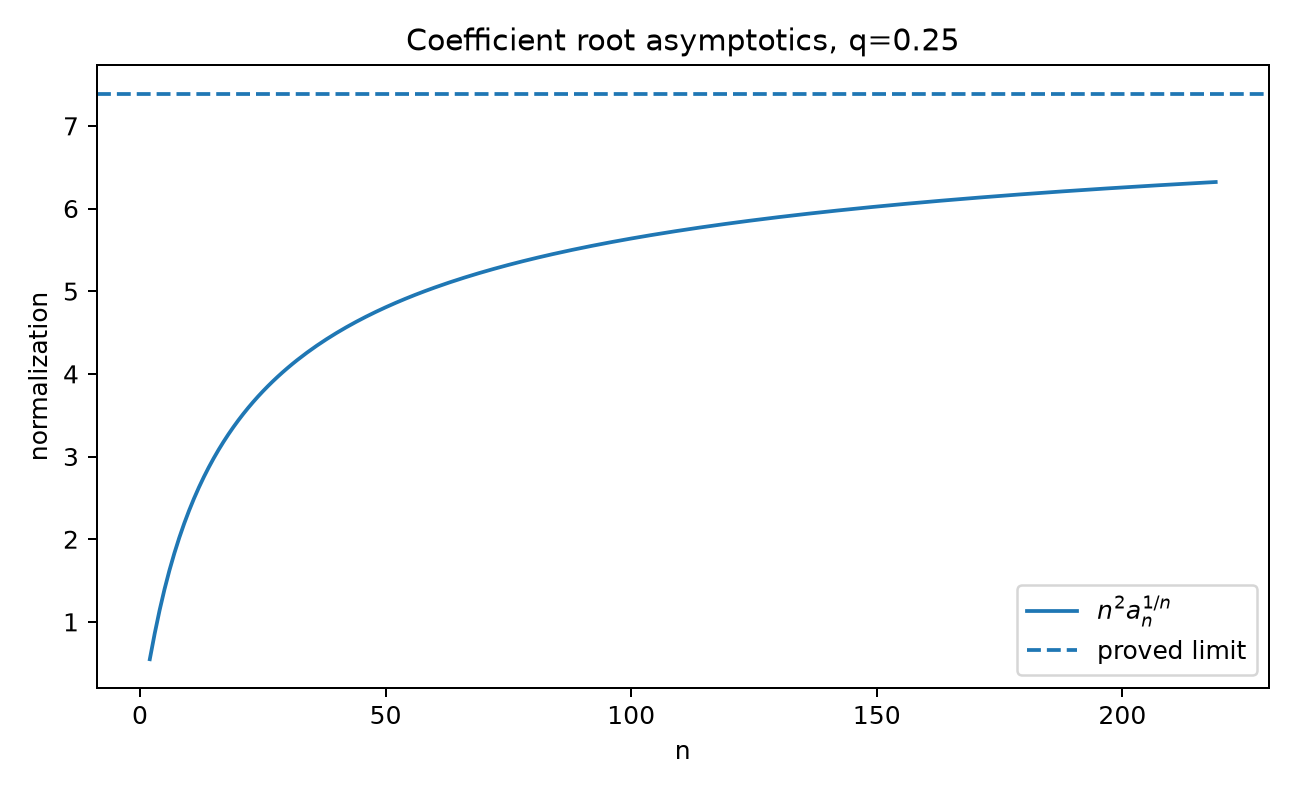
\includegraphics[width=0.82\textwidth]{figures/coefficient_root_asymptotics.png}
\caption{Slow convergence of $n^2a_n^{1/n}$ to $\EulerE^2$ in the dyadic case.  The logarithmic-square correction in \eqref{eq:log-an} explains the visible delay.}
\label{fig:root-asymptotic}
\end{figure}

\begin{figure}[htbp]
\centering
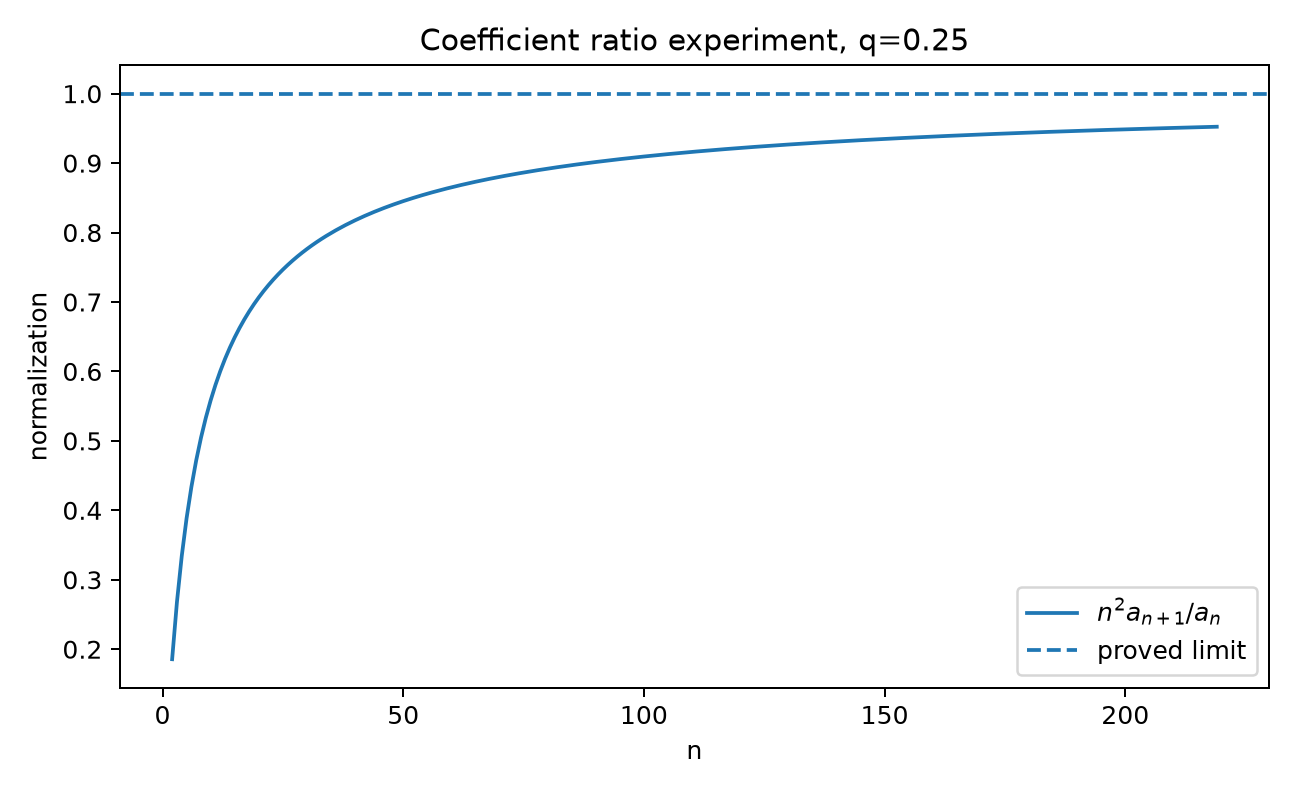
\includegraphics[width=0.82\textwidth]{figures/coefficient_ratio_asymptotics.png}
\caption{The ratio normalization $n^2a_{n+1}/a_n$ approaching the proved limit $1$ for $q=1/4$.}
\label{fig:ratio-asymptotic}
\end{figure}

Representative computed values are
\begin{center}
\begin{tabular}{rcc}
\toprule
$n$ & $n^2a_n^{1/n}$ & $n^2a_{n+1}/a_n$\\
\midrule
20 & 3.4359279255 & 0.7066033101\\
50 & 4.8047388703 & 0.8452331677\\
100 & 5.6370037156 & 0.9094953034\\
150 & 6.0236888401 & 0.9348387531\\
219 & 6.3204742781 & 0.9524028790\\
\bottomrule
\end{tabular}
\end{center}
The target values are $\EulerE^2\approx7.389056099$ and $1$.

\section{Structural consequences and interfaces with the existing corpus}\label{sec:interfaces}

\subsection{Why the $q$ here is the square of the dyadic $q$}

The finite Gaussian-binomial formulas in the repository naturally use base $1/2$, because they act on the dilation nodes $2^{-j}$.  The present product uses $q=1/4$ because the square-root substitution turns a sine factor into a power series in the square of that scale.  Thus the two $q$'s are not competing conventions:
\[
 \text{dilation scale }2^{-j}
 \quad\longmapsto\quad
 \text{spectral alphabet weight }(2^{-j})^2=4^{-j}.
\]
The Lambert denominator $1-4^{-m}$ in \eqref{eq:Pm-dyadic} is the even-moment shadow of the $1/2$-geometric refinement.

\subsection{Relation to the endpoint and inverse-Fabius asymptotics}

The endpoint analysis in the corpus finds a dominant Lambert-$W$ phase together with a periodic fluctuation in a logarithmic dyadic variable.  The coefficient problem here is a different asymptotic regime, but \eqref{eq:log-growth-refined} shows the same mechanism: the transition index
\[
 j\approx\frac{\log\sqrt t}{\log2}
\]
moves through an integer lattice as $t$ grows.  Its floor generates a bounded periodic remainder after the displayed quadratic and linear logarithmic terms are removed.  The coefficient saddle then samples that remainder near $\sqrt{t_n}\sim n$.  This predicts a log-periodic coefficient transseries, formulated precisely in \cref{conj:transseries}.

\subsection{Moment and Legendre interfaces}

The existing Legendre expansion of $\RvachevUp$ is linked to $(c_n)$ by a finite triangular transform, because each even Legendre polynomial is a linear combination of $1,x^2,\ldots,x^{2n}$.  Theorems \ref{thm:PF}, \ref{thm:multiplier}, and \ref{thm:moment-sandwich} therefore provide a new source of inequalities for every finite block of Legendre coefficients after conjugation by that triangular matrix.  Total positivity is not automatically preserved by an arbitrary basis change, so the strongest possible Legendre formulation remains open.  A concrete goal is to identify a sign-regular normalization of the monomial-to-Legendre matrix that transports selected Toeplitz minors to the even Legendre coefficient sequence.

\subsection{Operator meaning}

The multiplier theorem supplies an explicit hyperbolicity preserver attached to the up function:
\begin{equation}\label{eq:operator}
 \mathcal M_{\RvachevUp}\!\left(\sum_{n=0}^{d}u_nx^n\right)
 :=\sum_{n=0}^{d}\frac{4^nn!c_n}{(2n)!}u_nx^n.
\end{equation}
Every real-rooted input polynomial is sent to a real-rooted output polynomial.  This is an operator-theoretic statement about the moment sequence, not a property visible from the refinement differential equation alone.  The geometric family gives a continuous cone of such diagonal preservers indexed by $q\in(0,1)$.

\section{Conjectures}\label{sec:conjectures}

The following statements are supported by the proved structure and by numerical experiments, but they are not proved here.

\begin{conjecture}[Hermite universality for shifted Jensen polynomials]\label{conj:hermite}
Fix $0<q<1$ and $d\ge1$.  After the canonical affine rescaling determined by the first two logarithmic differences of
$\gamma_n(q)=n!a_n(q)$, the shifted Jensen polynomials
$J_{\gamma(q)}^{d,n}$ converge coefficientwise, and hence locally uniformly, to the degree-$d$ Hermite polynomial as $n\to\infty$.
\end{conjecture}

Exact hyperbolicity is already supplied by \cref{thm:jensen}; the conjecture concerns the finer geometry of the roots.  The asymptotic \eqref{eq:log-an} has the smooth log-polynomial shape that produces Hermite limits in many other sequences.  The dyadic periodic term should enter only at a lower normalization order.

\begin{conjecture}[Full log-periodic coefficient transseries]\label{conj:transseries}
For every $0<q<1$ there exist constants $A_q,C_q$, a real-analytic one-periodic function $\Omega_q$, and a complete expansion in descending powers of $n$ with polynomial coefficients in $\log n$, such that
\begin{align}
 \log a_n(q)
 ={}&2n-2n\log\!\left(\frac{2n}{\sigma_q}\right)
 -\frac{(\log n)^2}{2L_q}+A_q\log n+C_q\notag\\
 &+\Omega_q\!\left(\frac{\log n}{L_q}\right)
 +\sum_{r\ge1}\frac{Q_{q,r}(\log n,
 \Omega_q,\Omega_q',\ldots)}{n^r}.
 \label{eq:transseries-conj}
\end{align}
For $q=1/4$, the Fourier frequencies of $\Omega_q$ are integer multiples of $2\pi/\log2$.
\end{conjecture}

\begin{conjecture}[Phase duality with endpoint flatness]\label{conj:phase-duality}
In the dyadic case, the periodic function in \eqref{eq:transseries-conj} is obtained from the periodic Gamma--zeta fluctuation in the endpoint asymptotic of $\FabiusBounded(x)$ by an explicit saddle/Legendre transform, up to an elementary change of phase and normalization.
\end{conjecture}

This would make the coefficient asymptotic and the inverse-Fabius Lambert-$W$ asymptotic two dual projections of the same Mellin singularity lattice.

\begin{conjecture}[Arithmetic rigidity for rational geometric scale]\label{conj:arithmetic}
Let $q=A/B\in(0,1)$ be rational in lowest terms.  After multiplying $a_n(q)$ by an explicit product built only from $(B^m-A^m)$, Bernoulli denominators, and factorials for $m\le n$, the result is an integer.  For $q=1/4$, this normalization should admit a refinement whose odd-prime factors are controlled by the same Mersenne-type products that occur in exact Fabius values.
\end{conjecture}

The recurrence \eqref{eq:a-recurrence} proves rationality and gives a crude denominator bound; the conjecture asks for a sharp, cancellation-aware analogue of the known Fabius integrality phenomena.

\begin{conjecture}[Legendre sign regularity]\label{conj:legendre}
There is a diagonal sign and magnitude normalization of the even Legendre coefficient sequence of $\RvachevUp$ for which all contiguous minors up to each fixed order are eventually nonnegative.  Equivalently, a finite-order shadow of the PF$_\infty$ moment structure survives the monomial-to-Legendre basis transform.
\end{conjecture}

\section{Promising research directions}\label{sec:future}

\subsection{Formalization targets}

The shortest route into Lean is modular.
\begin{enumerate}[leftmargin=2.2em]
\item Formalize the Euler product \eqref{eq:sinh-product} and the double-product rearrangement \eqref{eq:H-double-product} under absolute local convergence.
\item Define finite spectral alphabets, prove total nonnegativity by products of bidiagonal Toeplitz matrices, and pass to limits one fixed minor at a time.
\item Import or prove the finite Pólya--Schur criterion needed for Jensen polynomials; the full classification theorem is not necessary if one works through finite truncations and Hurwitz limits.
\item The finite general-base multiplicity sum and digit-sum identity are now
formalized by the five-theorem API in \path{BaseDigitMultiplicity.lean}, for
all \(b>1\) and \(N\ge0\).  Still formalize the analytic identification of
those arithmetic multiplicities with zero orders; the sign interpolation
then additionally requires product convergence, the exact zero set,
continuity, and parity of zero crossings.
\item Formalize the exact coefficient recurrence \eqref{eq:a-recurrence}; it is algebraic once the logarithmic series is available.
\end{enumerate}
These items are substantially more tractable than formalizing the local central limit theorem.  The root limit can initially be recorded as an analytic theorem with a separate probability module.

\subsection{de Branges and desingularized zero sets}

The Cartwright function $\widehat{\RvachevUp}$ has the correct growth for de Branges-style analysis but the wrong zero geometry for the simplest sine-type machinery: dyadic collisions create unbounded multiplicity.  Two desingularizations are natural.  One may perturb the scales $2^{-j}$ to $2^{-j}\EulerE^{\varepsilon_j}$ with rationally independent $\varepsilon_j$, splitting all collisions while preserving type; or divide out a controlled canonical product encoding the excess multiplicities.  The question is whether either construction produces a Hermite--Biehler function whose de Branges space has a meaningful limit as the perturbation vanishes.

\subsection{Strict minors and tableaux}

Equation \eqref{eq:schur-minor} invites exact combinatorics.  Expanding a Schur specialization in the alphabet \eqref{eq:Aq} produces weighted semistandard tableaux with entries $(j,k)$ and weight $q^j/(\pi^2k^2)$.  Summing first over $k$ should yield multiple-zeta values; summing first over $j$ should yield rational functions of $q$.  Determining when the resulting multiple-zeta combinations collapse to rational multiples of powers of $\pi$ would connect total positivity to the arithmetic themes already prominent in the corpus.

\subsection{Asymptotic root processes}

The Jensen roots are exactly negative at every shift.  Their centered/scaled limiting process, the first periodic correction, and the dependence on $q$ are computationally accessible.  A useful experiment is to compute degrees $d=2,\ldots,20$ at shifts up to several thousand using the positive saddle recurrence rather than the cancellation-prone logarithmic recurrence.  One can then test whether the dyadic phase produces an oscillatory displacement of the Hermite zeros.

\subsection{Rational bases and automatic sign words}

The base-$b$ sign word in \eqref{eq:b-sign} is automatic: a finite automaton can track the required residue of $bN-s_b(N)$ while reading base-$b$ digits.  Classifying these words up to morphic equivalence, spectral type, subword complexity, and substitution rules would place the binary Thue--Morse theorem in a larger automatic family.  For nonintegral geometric scales, zero collisions largely disappear; the transition from automatic multiplicity words to simple quasi-periodic divisors is a natural deformation problem.

\subsection{Inverse and endpoint matching}

The coefficient saddle variable $t_n$ and the inverse-Fabius Lambert variable solve different stationarity equations.  Both can be expanded through Lambert $W$ after the logarithmic-square term is included.  A systematic comparison should reveal whether the two periodic phases are literally the same Mellin residue series or only share their frequency lattice.  This is the most direct bridge from the new total-positivity direction back to the corpus's strongest endpoint results.

\section{Numerical methodology and reproducibility}\label{sec:numerics}

The accompanying program \texttt{fabius\_frontier\_experiments.py} performs the following checks.
\begin{enumerate}[leftmargin=2.2em]
\item It computes exact $P_m$, $a_n$, $c_n$, and $\gamma_n$ with SymPy rational arithmetic and writes both CSV and LaTeX tables.
\item It evaluates \eqref{eq:a-recurrence} to order 220 with 1430 decimal digits.  This excessive precision is intentional: the recurrence alternates and suffers catastrophic cancellation even though the final coefficients are positive.
\item It compares the coefficient series with a direct 28-factor product at $x=0.1,1,10$.  The observed relative discrepancies are approximately $3.1\times10^{-19}$, $3.1\times10^{-18}$, and $3.1\times10^{-17}$, consistent with the omitted product tail.
\item It computes degree-five shifted Jensen roots at shifts $0,1,4,8,16,24$ with 70-digit root finding.  Every imaginary part is exactly reported as zero by the high-precision computation, and every real part is negative.
\item It writes the exact zero-count data $Z_+(M)=2M-s_2(M)$ through $M=4096$ and produces \cref{fig:zero-discrepancy}.
\end{enumerate}

The first degree-five Jensen polynomial has approximate roots
\[
 -20.5202748721,\quad-13.2270889615,\quad-8.0145285161,
 \quad-4.5386982674,\quad-1.5584201014.
\]
These computations are evidence and consistency checks; the real-rootedness claim itself is proved abstractly in \cref{thm:jensen}.

\section{Conclusion}

The imaginary square-root transform changes the viewpoint on the Fabius--Rvachev Fourier product.  What appears on the real axis as an oscillatory product with intricate dyadic cancellations becomes, in the new variable, a positive genus-zero product over an explicit spectral alphabet.  Five theories then meet at one formula:
\[
 \boxed{
 H(x)=\widehat{\RvachevUp}\!\left(\frac{\ImaginaryUnit\sqrt{x}}{\pi}\right)
 =\prod_{n=1}^{\infty}
  \left(1+\frac{x}{\pi^2n^2}\right)^{\nu_2(n)+1}
 =\sum_{n=0}^{\infty}\frac{4^nc_n}{(2n)!}x^n.}
\]
The left side remembers the compactly supported atomic function; the middle expression exposes the valuation-weighted divisor; the right side exposes the moments.  Laguerre--Pólya theory converts the divisor into a real-rootedness preserver, total positivity converts it into inequalities and positive minors, Bell polynomials convert its logarithm into exact recurrences, and Bernoulli tilting converts its coefficients into a local central-limit saddle.  Returning to the real Fourier axis, the same divisor makes the Thue--Morse sequence visible as a sign word.

This package overlaps the existing Laguerre--P\'olya, PF-infinity, shifted-Jensen, zero-count, and sign developments, while organizing them alongside additional Cartwright and deformation questions.  Its remaining frontier directions ask how coefficient asymptotics match the Lambert-$W$ endpoint phase, how Toeplitz minors transport toward Legendre coordinates, and how dyadic collisions might be desingularized toward de Branges spaces.  These questions are concrete enough for exact computation and formalization, but no package-wide novelty claim is intended.

\appendix
\section{A compact theorem dependency map}

\begin{center}
\begin{tabularx}{\textwidth}{p{0.25\textwidth}X}
\toprule
Input & Consequence \\
\midrule
Sinc Fourier product & Zero divisor, Cartwright type, sign interpolation.\\
Imaginary square-root substitution & Positive sinh product and moment coefficients.\\
Weierstrass product for $\sinh z/z$ & Explicit positive spectral alphabet.\\
Genus-zero positive product & Laguerre--Pólya type I.\\
Bidiagonal Toeplitz factorization & PF$_\infty$ and Schur-positive minors.\\
Pólya--Schur theorem & Multiplier sequence and all shifted Jensen hyperbolicity.\\
Degree-two Jensen hyperbolicity + Cauchy--Schwarz & Adjacent-moment sandwich.\\
Power sums of the alphabet & Lambert factors, zeta/Bernoulli recurrence, Bell formula.\\
Bernoulli tilt of the alphabet & Exact coefficient probability and saddle formula.\\
Geometric scales & Explicit growth, root limit, ratio limit, log-periodic frontier.\\
\bottomrule
\end{tabularx}
\end{center}

\section{First exact values}

For reference, the first terms are
\begin{align*}
 a_0&=1,& c_0&=1,&\gamma_0&=1,\\
 a_1&=\frac29,& c_1&=\frac19,&\gamma_1&=\frac29,\\
 a_2&=\frac{38}{2025},&c_2&=\frac{19}{675},&\gamma_2&=\frac{76}{2025},\\
 a_3&=\frac{2332}{2679075},&c_3&=\frac{583}{59535},&
 \gamma_3&=\frac{4664}{893025}.
\end{align*}
They satisfy both the source moment recurrence and the new Bernoulli recurrence \eqref{eq:c-Bernoulli}.

\section{Research-status ledger}

\begin{longtable}{p{0.43\textwidth}p{0.14\textwidth}p{0.348\textwidth}}
\toprule
Statement & Status & Basis \\
\midrule
\endhead
Zero multiplicity $\nu_2(N)+1$ & Proved & Direct factor count.\\
Exact count $2N-s_2(N)$ & Proved & Legendre digit-sum identity.\\
Thue--Morse sign interpolation & Proved & Parity of cumulative multiplicity.\\
Finite base-$b$ multiplicity/digit identity & Lean-proved arithmetic & \path{BaseDigitMultiplicity.lean}; every $b>1$ and $N\ge0$, with no analytic zero or sign claim.\\
Laguerre--Pólya type I & Proved & Genus-zero positive product.\\
PF$_\infty$ moments & Proved & Bidiagonal factorization / AESW.\\
Multiplier sequence & Proved & Pólya--Schur.\\
All shifted Jensen polynomials hyperbolic & Proved & Derivative closure of $\mathcal{LP}$.\\
Moment sandwich & Proved & Turán plus Cauchy--Schwarz.\\
Bernoulli/Bell recurrences & Proved & Logarithmic power sums.\\
Cartwright indicator & Proved & Directional product estimates.\\
Poisson-binomial saddle formula & Proved & Exponential tilting and local CLT.\\
Coefficient root and ratio limits & Proved & Saddle asymptotic plus log-concavity.\\
Hermite limit & Conjecture & Exact hyperbolicity and log-polynomial evidence.\\
Full periodic transseries & Conjecture & Geometric transition index and numerics.\\
Endpoint/coefficient phase duality & Conjecture & Shared Mellin frequency lattice.\\
Sharp rational-$q$ integrality & Conjecture & Exact rational recurrence.\\
Legendre sign regularity & Conjecture & Triangular moment transform.\\
\bottomrule
\end{longtable}

\begin{thebibliography}{99}
\bibitem{Arias1982}
J. Arias de Reyna,
\emph{An infinitely differentiable function with compact support: definition and properties},
arXiv:1702.05442, English translation of Rev. Real Acad. Cienc. Exact. Fís. Natur. Madrid 76 (1982), 21--38.

\bibitem{AriasArithmetic}
J. Arias de Reyna,
\emph{Arithmetic of the Fabius function},
arXiv:1702.06487, 2017 (repository source updated 2026).

\bibitem{AESW}
M. Aissen, A. Edrei, I. J. Schoenberg, and A. Whitney,
\emph{On the generating functions of totally positive sequences},
Proc. Natl. Acad. Sci. USA 37 (1951), 303--307.

\bibitem{Edrei}
A. Edrei,
\emph{On the generating functions of totally positive sequences II},
J. Analyse Math. 2 (1952), 104--109.

\bibitem{PolyaSchur}
G. Pólya and J. Schur,
\emph{Über zwei Arten von Faktorenfolgen in der Theorie der algebraischen Gleichungen},
J. Reine Angew. Math. 144 (1914), 89--113.

\bibitem{Levin}
B. Ya. Levin,
\emph{Distribution of Zeros of Entire Functions},
American Mathematical Society, revised edition, 1980.

\bibitem{GriffinOnoRolenZagier}
M. Griffin, K. Ono, L. Rolen, and D. Zagier,
\emph{Jensen polynomials for the Riemann zeta function and other sequences},
Proc. Natl. Acad. Sci. USA 116 (2019), 11103--11110; arXiv:1902.07321.

\bibitem{OSullivan}
C. O'Sullivan,
\emph{Limits of Jensen polynomials for partitions and other sequences},
arXiv:2108.06775, 2021.

\bibitem{Simonelli}
I. Simonelli and L. D. Simonelli,
\emph{Local limit theorems for Poisson's binomial in the case of infinite expectation},
arXiv:1803.04153, 2018.

\bibitem{ProveIt}
V. Reshetnikov,
\emph{ProveIt: Analysis/FabiusFunction}, GitHub repository,
commit \texttt{fc4b8868fcf57cc534d22f438d940ec65ebbe767}, 30 August 2026.
\end{thebibliography}

\end{document}
